\section{Programm}
\subsection{Einleitung}
Um die Methoden der Threads in einer Realen Situation zu nutzen, habe ich mich entschlossen ein Programm, welches stark von Threads profitieren kann, zu programmieren.  

Ich habe mich für ein Programm eintscheiden, mit dem man ein Bild mit vielen weiteren Bildern rekrieren kann. Es wird demnach ein Mosaik aus Bildern erstellt.

\begin{figure}[h]
    \centering
    \subfloat[\centering Input]{
        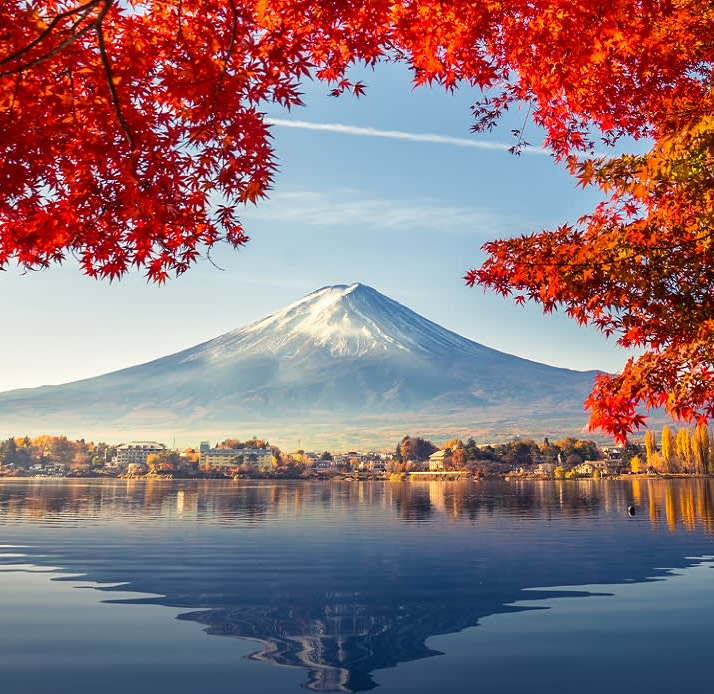
\includegraphics[height=5cm]{images/Source_100x100}
    }
    \subfloat[\centering Output]{
        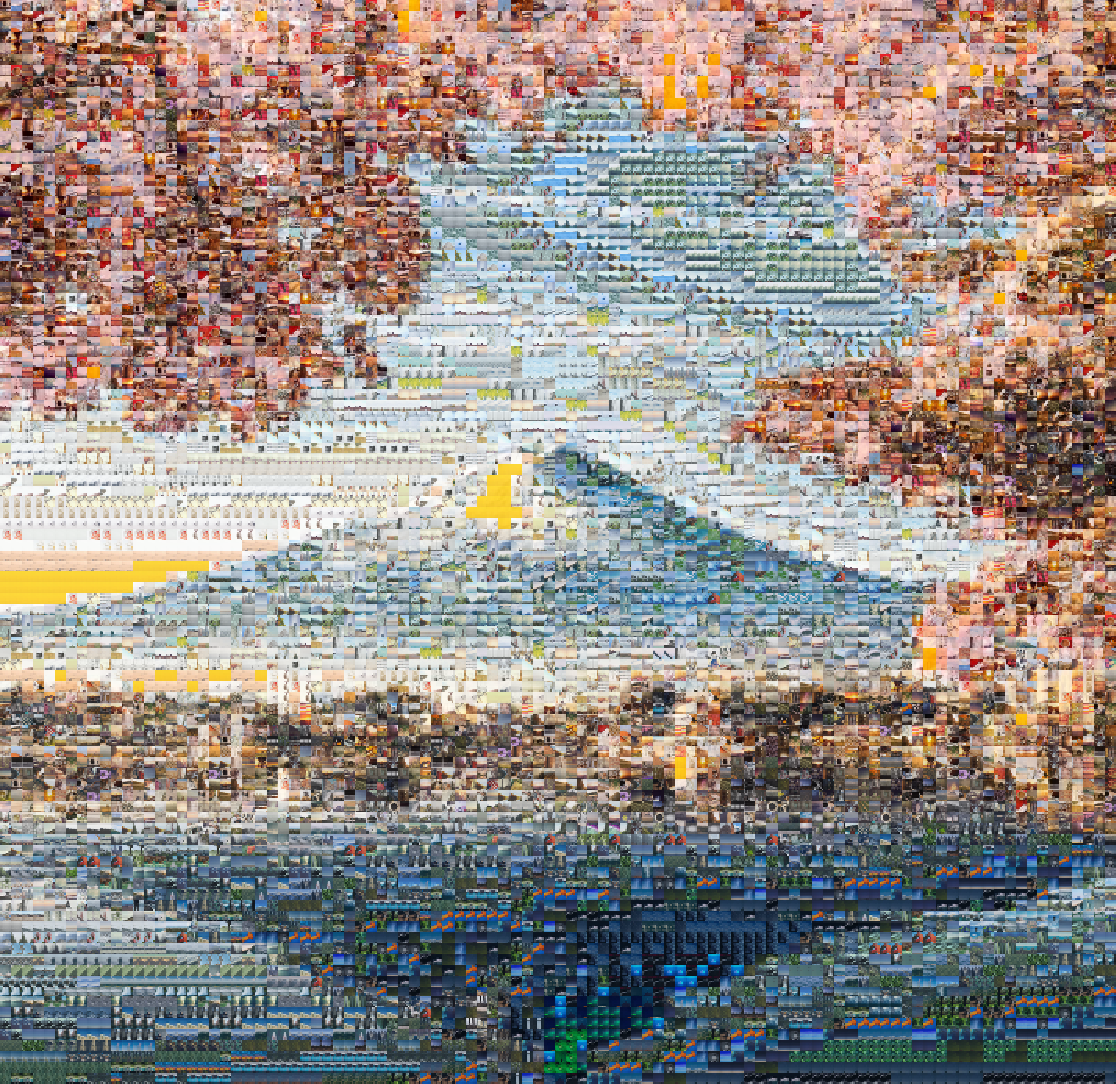
\includegraphics[height=5cm]{images/Render_100x100}
    }
    \caption[Programm Funktion]{Funktionsweise des Programmes}
\end{figure}

Die anwendung von Threads kommt in dem Programm in vielen Stellen vor. Im folgen werde ich mich auf den Algorythmus der Bild analyse und verarbeitung beziehen. Andere aspekte, wie die implementation des Testmodus und andere Features, die in der App vorhanden sind, werden kurz im Anhang erwähnt.

\newpage
\subsection{Idee}
In der genaueren Betrachtung, muss das Programm das eingegebene Bild vereinfachen. Dies wird durch eine Unterteilung des Bildes in Sektoren erreicht. Die Sektoren sind auch die zukünftigen Stellen für die ausgewählten Bilder. Es wird die durchschnittliche Farbe der Sektoren berechnet. Das selbe vorgehen wird auch auf die ausgewählten Bilder angewendet. Dabei ist ein Bild ein Sektor. Dieses vorgehen erlaubt es auch, Datenbanken (im JSON-Format) zu erstellen, da sich die durchschnittliche Farbe der ausgewählten Bilder nicht ändern wird. Anschließend wird mit einem Algorithmus die passenden Bilder für die einzelnen Sektoren berechnet. Dabei unterliegt der Algorithmus der Beschränkung, dass der Nutzer wählen kann, wie häufig ein Bild vorkommen darf. Nach dem berechnen der benötigten Bilder müssen diese für die Verwendung angepasst werden. Es soll schließlich nicht ein 10x10px großer Teil aus einem 4000x3000px Bild verwendet werden. Dazu wird das Bild erst Skaliert und schließlich zurechtgeschnitten. Dabei liegt der Fokus darauf, immer die Mitte des Bildes zu treffen. Das Programm arbeitet die Schritte nachfolgend ab und in dieser Reihenfolge werde ich das Programm nachfolgend erklären.

\subsection{Implementation in Java}
\subsubsection{Berechnen der Sektionen}
Das berechnen der Sektionen ist eigentlich ziemlich geradeaus. Die Größe des Bildes ist bekannt und in wie viele Teile dieses aufgeteilt werden soll. Dazu wird zb. die Breite des Bildes mit der vertikalen Anzahl an Sektoren geteilt. Das Problem liegt darin, dass die Breite oder Höhe des Bildes nicht ein redundant von den gewünschten Sektoren ist. Um das Problem anzugehen wird ersterer Schritt nur mit Integers ausgeführt und der Rest berechnet wird. Übergeblieben sind wie viele Spalte auf der X- und Y-Achse gemacht müssen und der Rest der über bleibt. Im nächsten Schritt werden die Größen der Sektoren in Pixeln berechnet. Dies erfolgt dadurch, dass zwei Arrays für die X- und Y-Achse mit der Anzahl an benötigten Spalten gefüllt werden. Ein weiteres Array mit der Anzahl der Spalten wird aufsteigend nummeriert. Das Array wird von einer Methode gemischt. Eine Abschließende Schleife wird mit der Anzahl des Restes wiederholt und bei jedem Schritt wird ein dann zufälliger Wert aus den Array als Index für das Array mit der Größe der Sektoren genutzt. Das nun zufällige Segment wird um 1 erhöht. Die berechneten Werte werden in einem ``splitObj'' gespeichert. In diesem werden die Werte in unterschiedlichsten Arten wie z.B. Koordinaten gespeichert. 

Diese Koordinaten werden im nächsten Schritt benutzt, um ein zweidimensionales Array an ``BufferedImages'' aus dem Original Bild zu extrahieren. Dazu wird die ``getSubimage()'' Methode der Klasse ``BufferedImage'' verwendet.

\subsubsection{Berechnen der durchschnittlichen Farbe}
Das berechnen der durchschnittlichen Farbe von Segmenten und Bildern ist die erste Funktion, welche Threads nutzt. Implementationen von mir, welche Threads benutzen, bestehen meistens aus zwei Klassen. Eine Klasse, welche die Threads erstellt und verwaltet und eine weitere, welche den Code zum berechnen der jeweiligen Anforderung hat. In diesem Falle das Berechnen der durchschnittlichen Farbe. Die Klasse ``computeAverageColor'' besteht aus zwei Methoden. Eine zum Berechnen der Segmente und eine weitere für die gewählten Bilder. Der einzige Unterschied der beiden Methoden ist eine Sicherheitsfunktion in der Methode der Bilder welche wartet, bis genügend RAM verfügbar ist, bevor es das Bild in den RAM läd. Dies ist wichtig, da mehrere Threads gleichzeitig die Bilder im RAM zum Berechnen halten müssen. Je nach RAM Configuration und Bildergröße kann dies zu Komplikationen führen. Um zuverlässig die Größe des Bildes zu berechnen, kann nicht einfach die Dateigröße verwendet werden. Durch Komprimierungsverfahren wie jpg und png kann die Dateigröße eines Bildes um das 10-fache verkleinern. Um die wirkliche Größe zu berechnen, müssen die Dimensionen mal die Farbtiefe gerechnet werden. Die verwendeten BufferedImages haben eine Farbtiefe von 4byte oder 32bit. Um die Dimensionen eines Bildes auszulesen, ohne das gesamte Bild in den Speicher laden zu müssen, wird die ``ImageIO'' Klasse von java genutzt. Die ``ImageIO'' KLasse bietet eine Methode, mit welcher alle ``ImageReader'' eines Bildes erstellt werden. Ein ``ImageReader'' benötigt lediglich die Metadaten eines Bildes, welche nur einen Bruchteil der Dateigröße einsprechen, um die Dimensionen des Bildes zu lesen. Jeder der Threads ruft die Methode ``getAverage()'' der Klasse ``calculateAverage'' auf. Die Methode verlangt ein ``BufferedImage'' und ein enum ``calculateAverage.Method'', welches unterschiedliche Genauigkeitsstufen zum berechnen beinhaltet. Innerhalb der Methode ``getAverage()'' wird erst mit Hilfe des enums ein int definiert, welches beschreibt wie die nachfolgenden for-Schleifen erhöht werden. Weiterhin gibt es dre ``long''. Diese speichern den gesamten rot, blau und grün wert. Anschließend wird das Bild in der vorherigen definierten Schrittgröße durchgegangen und die rot, grün und blau werte des Pixels gespeichert. Zum Schluss wird ein neues ``Color'' Object mit den gesammelten werden geteilt durch die Anzahl der Pixel.

\subsubsection{Erstellen einer Datenbank}
Dieser Schritt wird immer dann durchgeführt, wenn im Programm Bilder ausgewählt wurden, oder eine speicherbare Datenbank erstellt wird. Wenn Datenbanken ausgewählt wurden, wird die eventuell erstellte Datenbank diesen hinzugefügt. Die Klasse ``DatabaseObj'' benötigt zwei Argumente. Eine Liste an Speicherorten der jeweiligen Bilder und ein Array an berechneten durchschnittlichen Farben. Innerhalb des ``DatabaseObj'' werden die beiden Werte der Listen in ``fileAndColor'' Objekten gespeichert. Wie der Name impliziert beinhalten die Objekte den Pfad des Bildes und den dazugehörigen Farbwert. Durch dieses Vorgehen kann ein BinarySort Algorithmus aus das neue Array angewendet werden. dazu hat die ``fileAndColor'' Klasse das ``Comparable'' interface implementiert. Für spätere Verwendung gibt es in den Objekten auch noch einen Zähler, welcher speichert, wie häufig das Bild in der Berechnung verwendet wurde. Alle Variablen der Klasse ``fileAndColor'' sind durch getter- setter-Methoden aufzurufen. Diese habe jedoch die Besonderheit, dass sie das ``synchronized'' Schlüsselwort besitzen (Hyperlink zu Kapitel Threads).
\bigskip
\newline
Besonders werde ich auf die Methode ``compareTo()'', des Interfaces Comparable eingehen. In der Methode werden zwei Farben verglichen. Welche größer und kleiner ist. Die Schwierigkeit liegt darin ein Ergebnis zu bestimmen, wenn vier Werte verglichen werden müssen. Der alpha-Wert, rot-Wert, grün-Wert und blau-Wert. Um ein einfachen und zuverlässigen Vergleich zu machen, nutze ich die Methode ``getRGB()'' der ``Color'' Klasse. Interessant ist jedoch, was diese Methode macht. In der Klasse ``Color'' werden alle vier Werte in einem einzigen Integer gespeichert. Das liegt an der Genauigkeit, womit Farben gemischt werden. Jeder Wert befindet sich in einem Bereich von 0 bis 255. Dies entspricht genau einem Byte. Ein Integer wiederum besteht aus vier Bytes. Die vie Farbwerte werden sozusagen in die vier Bytes des Integers eingesetzt. In der Reihenfolge ``ARGB''.\\
\begin{figure}[h]
    \centering
    \begin{tabular}{c | c | c | c || c}
        alpha(255) & rot(224) & grün(64) & blau(16) & \tikz \definecolor{dkOrange}{rgb} {0.88,0.25,0.06} \fill [dkOrange] (0, 0) rectangle (10pt, 10pt); \\
        \hline
        11111111 & 11100000 & 01000000 & 00010000 & -2080752
    \end{tabular}
\end{figure}
\\Durch dieses Vorgehen wird aus vier Werten ein zuverlässiger Wert erstellt, welcher zum sortieren geeignet ist.

\newpage

\subsubsection{Berechnen der besten Bilder}
Das Berechnen der besten Bilder für die jeweiligen Sektoren wird in der Klasse ``compareColor'' mit der Methode ``compare()'' ausgeführt. Die Methode gibt ein zweidimensionales ``File''-Array zurück. Dies steht dabei für die einzelnen Sektoren. Innerhalb der Methode wird für jeden Sektor ein ``Runnable'' erstellt. (siehe Kapitel Threads). Da es ein Limit für die Verwendung der Bilder gibt, sollen diese gleichmäßig verteilt werden. Um einen solchen Effekt zu erhalten wird eine Liste an ``Runnables'' erstellt und gemischt.

\begin{figure}[h]
    \centering
    \subfloat[\centering ohne mischung]{
        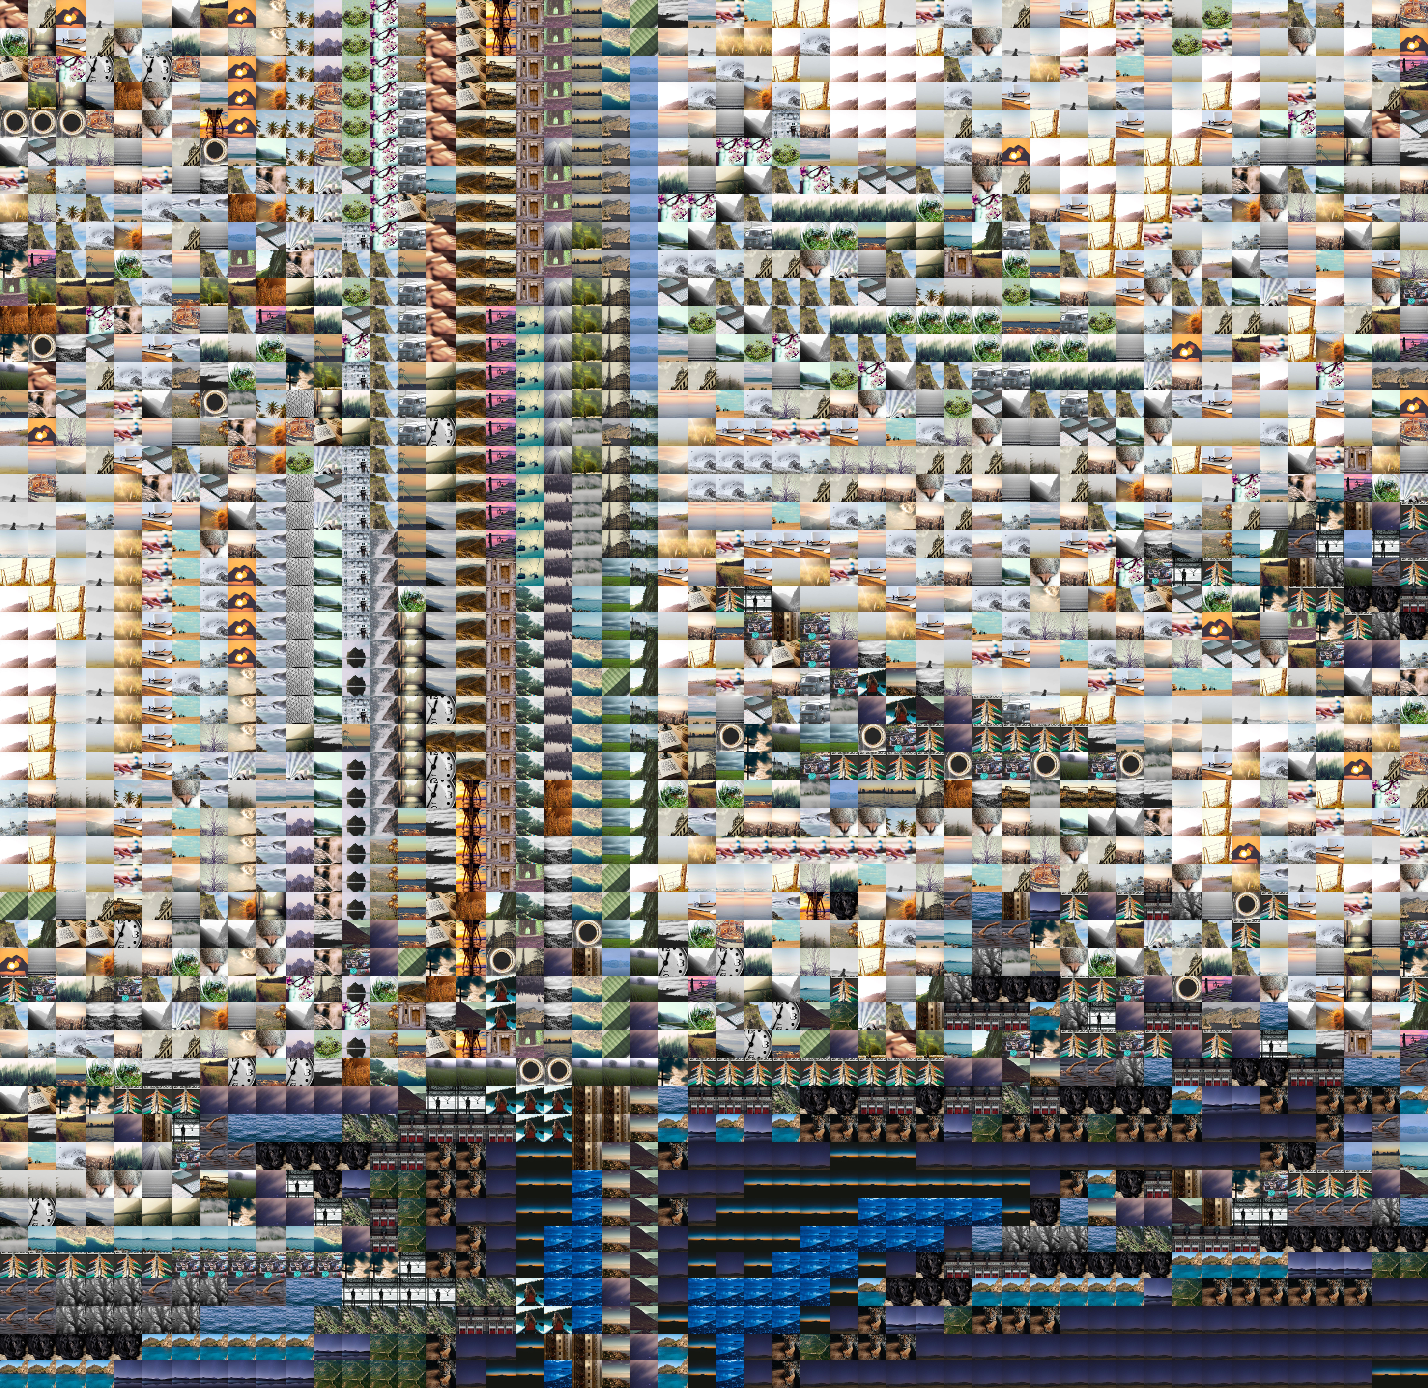
\includegraphics[height=5cm]{images/BadExample_Lines.png}
    }
    \subfloat[\centering mit mischung]{
        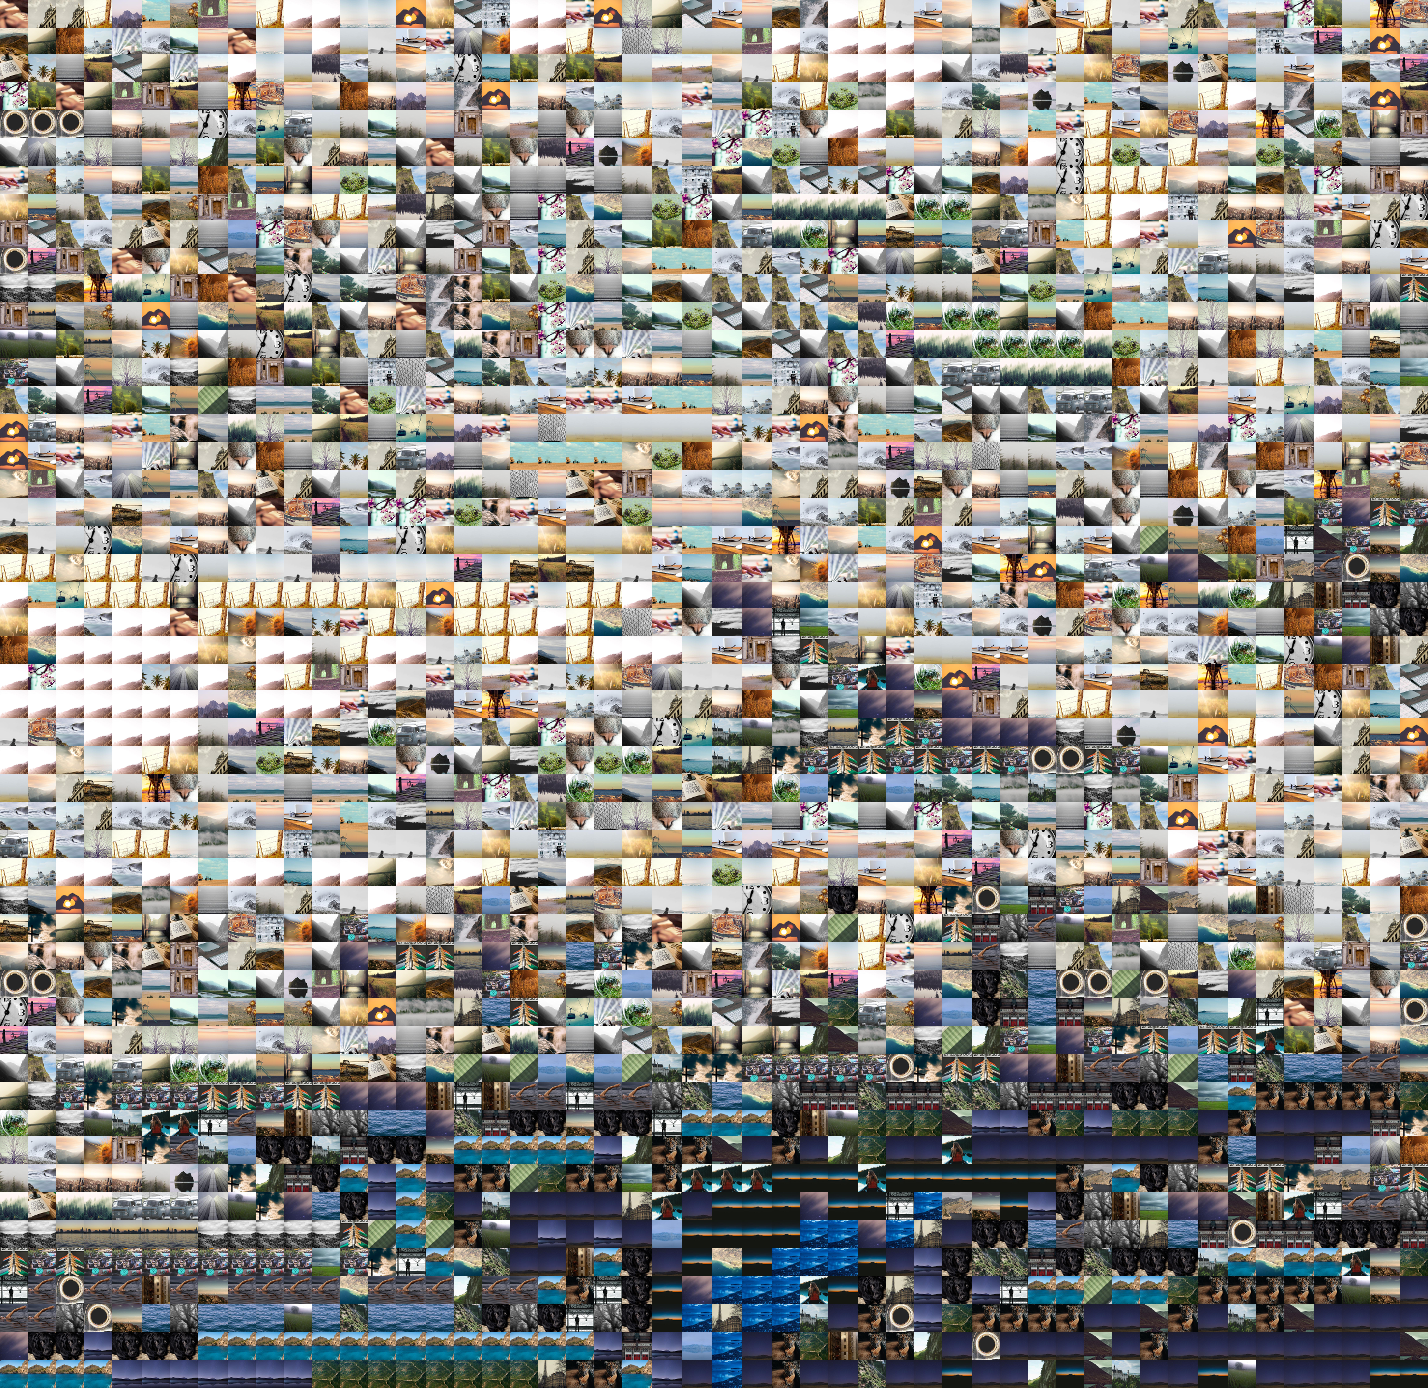
\includegraphics[height=5cm]{images/GodExample_NoLines.png}
    }
    \caption[Beste Bilder]{Unterschied zwischen mischen und nicht mischen}
\end{figure}

\begin{sloppypar}
Jeder ``Runnable'' sucht demnach nach dem besten Bild, welches noch verfügbar ist. Es werden dazu alle vorhandenen Datenbanken durchgegangen und für jede einzelne das beste Bild gesucht. Die besten aus alles Datenbanken werden dann verglichen und der beste wird gewählt. Um die beste Farbe einer Datenbank zu berechnen kann die java Methode ``Arrays.binarySearch'' verwendet werden. Diese Methode findet nicht nur den gleichen Wert, sondern auch einen index, an dem es den gesuchten Wert einsetzen würde. Anhand von dem Index wird dann im Array jeweils das nächste beste Bilde, welches noch nicht zu häufig verwendet wurde, gesucht. Die beiden gefundenen Werte, werden auf nähe zum gesuchten Wert überprüft. Der nähere wird dementsprechend auserwählt.
\end{sloppypar}

\newpage

\subsubsection{Skalieren der Bilder}
Das Skalieren der Bilder ist in drei Schritte einzuteilen. Das Management der Bilder, Berechnen der Zielgröße und das Skalieren an sich. Ich werde auf jeden Bereich individuell eingehen.

\paragraph{Management}
Da Ein Bild mehrfach ausgewählt werden kann, ist es wichtig ein Management System zu haben, welches verhindert, dass das selbe Bild nicht häufiger als nötig skaliert wird. Das Skalieren ist der Zeitaufwendigste Prozess, daher sollte dieser minimiert werden. Jedes Bild kann in vier unterschiedlichen Größen verwendet werden. Die Größen kommen aus dem in (siehe Berechnen der Sektionen) beschriebenen vorgehen. Werden die Bilder nur in einer einheitlichen Größe skaliert Entstehen schwarze Linien im Bild.

\begin{figure}[h]
    \centering
    \subfloat[\centering ohne mehrfach Skalierung]{
        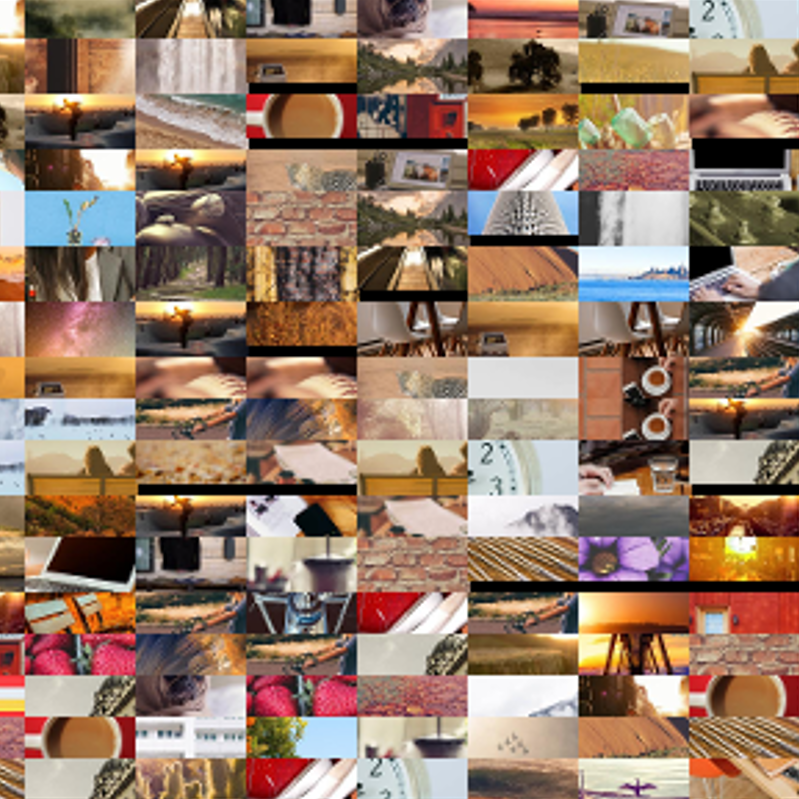
\includegraphics[height=5cm]{images/BadExample_BlackLines.png}
    }
    \subfloat[\centering mit mehrfach Skalierung]{
        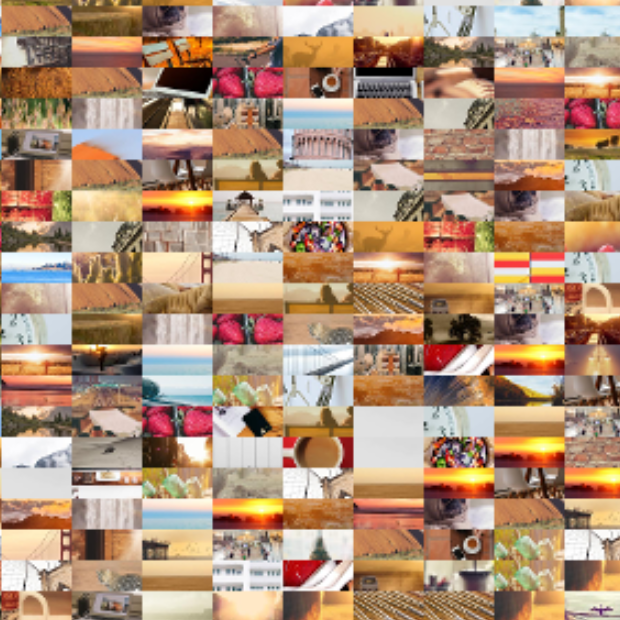
\includegraphics[height=5cm]{images/GodExample_NoBlackLines.png}
    }
    \caption[Schwarze Linien]{vierfache Skalierung der Bilder}
\end{figure}

Beim Managen wird demnach überprüft, ob ein bestimmtes Bild schon in der jeweiligen Größe vorhanden ist. Dazu wird eine Instanz der Klasse ``ScaledImages'' erzeugt. Diese Instanz fungiert als gemeinsamer Speicherort aller skalierten Bilder. Die Klasse hat ein zweidimensionales Array des Types ``ImageWithName'' und eine Methode ``exists()''. Die Methode ``exists()'' sucht mithilfe von dem Pfad des Bildes und den gewünschten Dimensionen in dem Array nach bereits skalierten Bildern. In dem Fall, dass etwas gefunden wird, werden die Koordinaten des gefunden Bildes zurückgegeben. Der Skalier-Thread speichert dan eine Referenz auf das gefundene Bild ab.
\medskip
\newline
Ein Problem beinhaltet das System jedoch noch. Es könnte zu der Situation kommen, dass mehrere Threads gleichzeitig mit dem gleichem Bildauftrag gestartet werden. Anfangs überprüft jeder Thread, ob sie arbeiten dürfen, oder das gewünschte Bild noch nicht existiert. Alle Threads werden davon ausgehen, dass die Arbeiten dürfen, da das Skalieren des Bildes und Speichern dessen vergleichsweise länger dauert als einen neuen Thread zu starten. Doch dadurch werden nicht nur Ressourcen unnütz verbraucht, sondern auch Fehler in der Bilddatei können entstehen, da mehrere Threads gleichzeitig eine Datei auslesen.

\begin{figure}[h]
    \centering
    \begin{minipage}{89mm}
        \fontsize{10pt}{11pt}\selectfont% or whatever fontsize you like
        \def\svgwidth{8cm}
        \input{images/Manager_Threads.pdf_tex}
    \end{minipage}
    \begin{minipage}{1\textwidth-91mm}
        1. Überprüfen, ob die Bilder schon vorhanden sind.\\
        2. Schreiben des Bildes in das Array.
    \end{minipage}
    \caption[Thread und Manager]{Threads mit Manager}
\end{figure}

Um ein solches Verhalten zu verhindern, versucht ein Thread ein Bild zu reservieren, wenn es laut Manager frei ist. Ein Reserviertes Bild, wird als bereits existierendes gewertet. Das Referenz System funktioniert weiterhin, da 